\begin{frame}[ctb!]
\frametitle{Clay GDSM Solubility Sensitivity}
For solubility limits above the threshold, increase to the limit had no effect on the peak dose. This demonstrates the 
situation in which the solubility limit is so high that even complete 
dissolution of the waste inventory into the pore water is insufficient to reach 
the solubility limit.
\begin{figure}[htb!]
\centering
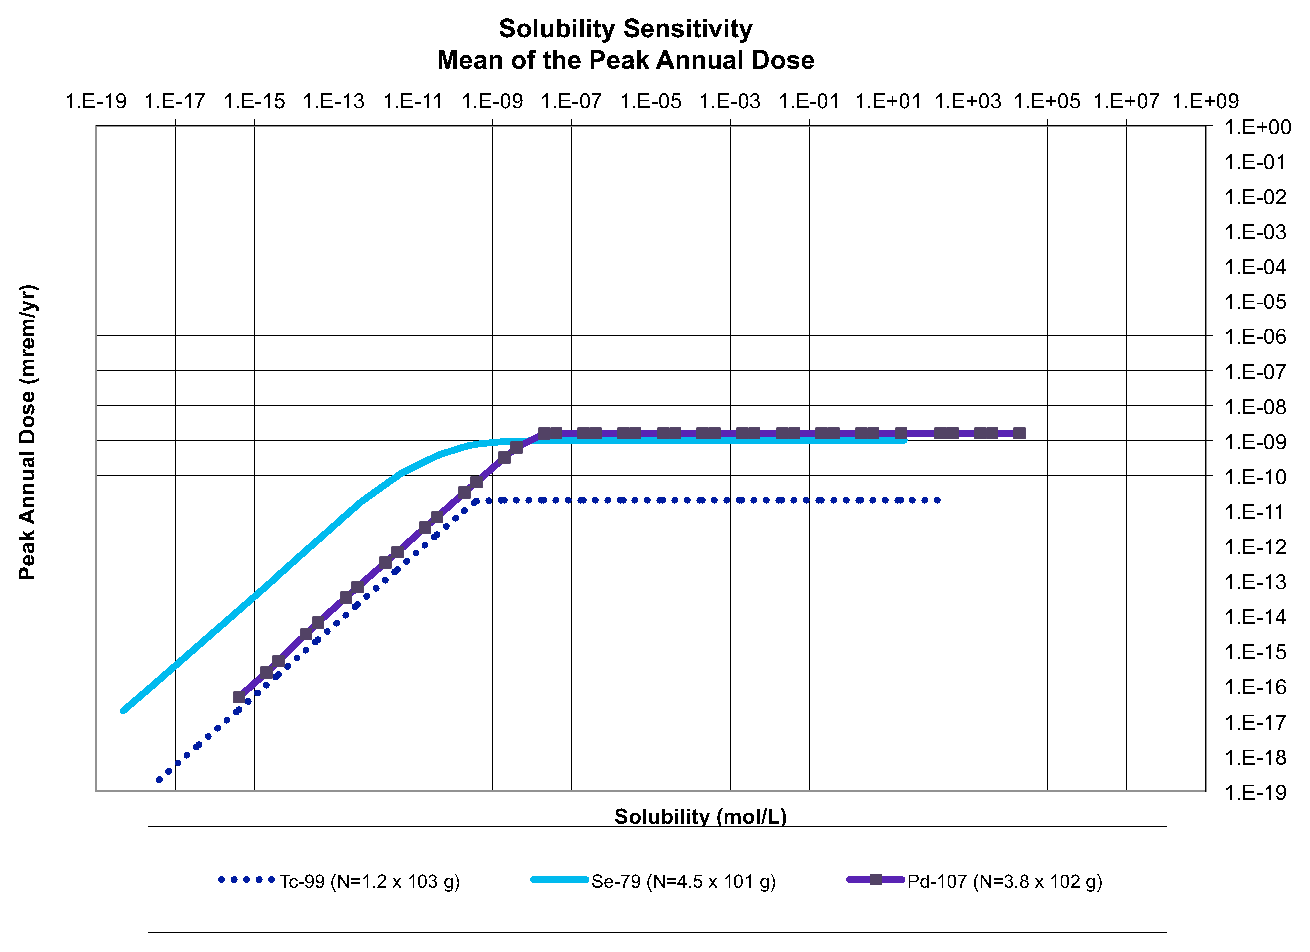
\includegraphics[width=0.7\linewidth]{./nuclide_demonstration/Solubility_Summary_Sol.eps}
\caption{Solubility limit sensitivity. The peak annual dose due to an inventory, 
$N$, of each isotope.}
\label{fig:SolSum}
\end{figure}
\end{frame}
